%% Based on a TeXnicCenter-Template by Tino Weinkauf.
%%%%%%%%%%%%%%%%%%%%%%%%%%%%%%%%%%%%%%%%%%%%%%%%%%%%%%%%%%%%%

%%%%%%%%%%%%%%%%%%%%%%%%%%%%%%%%%%%%%%%%%%%%%%%%%%%%%%%%%%%%%
%% HEADER
%%%%%%%%%%%%%%%%%%%%%%%%%%%%%%%%%%%%%%%%%%%%%%%%%%%%%%%%%%%%%
\documentclass[a4paper,oneside,9pt]{article}

% Alternative Options:
% use articl or report (report for longer documents)
%	Paper Size: a4paper / a5paper / b5paper / letterpaper / legalpaper / executivepaper
% Duplex: oneside / twoside
% Base Font Size: 10pt / 11pt / 12pt


%% Language %%%%%%%%%%%%%%%%%%%%%%%%%%%%%%%%%%%%%%%%%%%%%%%%%
\usepackage[USenglish]{babel} %francais, polish, spanish, ...
\usepackage[T1]{fontenc}
\usepackage[ansinew]{inputenc}

\usepackage{lmodern} %Type1-font for non-english texts and characters

\usepackage{color}
\usepackage{xcolor}
\usepackage{listings}
\usepackage{multirow}
\usepackage{footnote}

%% Packages for Graphics & Figures %%%%%%%%%%%%%%%%%%%%%%%%%%
\usepackage{graphicx} %%For loading graphic files
%\usepackage{subfig} %%Subfigures inside a figure
%\usepackage{tikz} %%Generate vector graphics from within LaTeX

%% Please note:
%% Images can be included using \includegraphics{filename}
%% resp. using the dialog in the Insert menu.
%% 
%% The mode "LaTeX => PDF" allows the following formats:
%%   .jpg  .png  .pdf  .mps
%% 
%% The modes "LaTeX => DVI", "LaTeX => PS" und "LaTeX => PS => PDF"
%% allow the following formats:
%%   .eps  .ps  .bmp  .pict  .pntg


%% Math Packages %%%%%%%%%%%%%%%%%%%%%%%%%%%%%%%%%%%%%%%%%%%%
\usepackage{amsmath}
\usepackage{wasysym}
\usepackage{amsthm}
\usepackage{amsfonts}
%\usepackage{url}
\usepackage{hyperref} 
\usepackage{geometry}
\usepackage{subfig}
\usepackage{verbatim} 
%%this sets up the margins
\geometry{left=2cm,right=2cm,bottom=2cm,top=2cm}%\geometry%{left=3.0cm,right=2.5cm,bottom=3cm,top=3cm}

\usepackage{natbib}

%% Line Spacing %%%%%%%%%%%%%%%%%%%%%%%%%%%%%%%%%%%%%%%%%%%%%
\usepackage{setspace}
%\singlespacing        %% 1-spacing (default)
\onehalfspacing       %% 1,5-spacing
%\doublespacing        %% 2-spacing


%% Other Packages %%%%%%%%%%%%%%%%%%%%%%%%%%%%%%%%%%%%%%%%%%%
%\usepackage{a4wide} %%Smaller margins = more text per page.
%\usepackage{fancyhdr} %%Fancy headings
%\usepackage{longtable} %%For tables, that exceed one page


%%%%%%%%%%%%%%%%%%%%%%%%%%%%%%%%%%%%%%%%%%%%%%%%%%%%%%%%%%%%%
%% Remarks
%%%%%%%%%%%%%%%%%%%%%%%%%%%%%%%%%%%%%%%%%%%%%%%%%%%%%%%%%%%%%
%
% TODO:
% 1. Edit the used packages and their options (see above).
% 2. If you want, add a BibTeX-File to the project
%    (e.g., 'literature.bib').
% 3. Happy TeXing!
%
%%%%%%%%%%%%%%%%%%%%%%%%%%%%%%%%%%%%%%%%%%%%%%%%%%%%%%%%%%%%%

%%%%%%%%%%%%%%%%%%%%%%%%%%%%%%%%%%%%%%%%%%%%%%%%%%%%%%%%%%%%%
%% Options / Modifications
%%%%%%%%%%%%%%%%%%%%%%%%%%%%%%%%%%%%%%%%%%%%%%%%%%%%%%%%%%%%%



%\input{options} %You need a file 'options.tex' for this
%% ==> TeXnicCenter supplies some possible option files
%% ==> with its templates (File | New from Template...).

%%%%%%%%%%%%%%%%%%%%%%%%%%%%%%%%%%%%%%%%%%%%%%%%%%%%%%%%%%%%%
%% SOME STUFF FOR NICE CODE LISTINGS
%%%%%%%%%%%%%%%%%%%%%%%%%%%%%%%%%%%%%%%%%%%%%%%%%%%%%%%%%%%%%

\usepackage{caption}
\DeclareCaptionFont{white}{\color{white}}
\DeclareCaptionFormat{listing}{\colorbox{gray}{\parbox{\textwidth}{#1#2#3}}}
\captionsetup[lstlisting]{format=listing,labelfont=white,textfont=white}

%%%%%%%%%%%%%%%%%%%%%%%%%%%%%%%%%%%%%%%%%%%%%%%%%%%%%%%%%%%%%
%% DOCUMENT
%%%%%%%%%%%%%%%%%%%%%%%%%%%%%%%%%%%%%%%%%%%%%%%%%%%%%%%%%%%%%
\begin{document}

\pagestyle{plain} %No headings for the first pages.


%% Title Page %%%%%%%%%%%%%%%%%%%%%%%%%%%%%%%%%%%%%%%%%%%%%%%
%% ==> Write your text here or include other files.

%% The simple version:
\title{Turbo2: First experiments with changes in abundance and isotopic signal}
\author{Dominik H\"ulse} % \\Candidate number: 52743
\date{05. June 2018} %%If commented, the current date is used.
\maketitle


\section{TURBO2: Very brief model description and experiment setup}\label{Intro_TURBO2} % and model comparison
\subsection{The model:}
TURBO2 simulates the effect of bioturbation on single sediment particles \citep{trauth_turbo2:_2013}. It is a mixed layer model with instantaneous, homogenous mixing (Fig. \ref{fig:TURBO2_schematic}).
The mixing depths can vary along the length of the core. TURBO2 simulates signal distortions of isotopic signals from stratigraphic carriers (e.g. forams). It can help to recognize distortions and uncertainties 
caused by bioturbation in combination with low sedimentation rates and low sample sizes of foraminifera shells used for isotope measurements.\\

\begin{figure}[hbp]
\begin{center}
	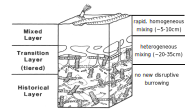
\includegraphics[width=0.6\textwidth]{../figures/Sediment_column.pdf}
	\caption{Copied from \citet{trauth_turbo2:_2013}: Generalized burrow stratigraphy in oxygenated pelagic sediments according
to Savrda et al. (1991) and Savrda (1992). The surface mixed layer (typically 5--10 cm thick) represents an interval of rapid and complete biogenic homogenization.
The transition layer, a zone of heterogeneous mixing that extends to subsurface depths of 20--35 cm, is characterized by burrows produced by organisms that live or
feed at greater depths in the substrate (i.e. below the mixed layer). With continued sediment accretion and associated upward migration of the mixed and transition
layers, sediment passes out of the actively bioturbated zone into a historical layer, in which no new disruptive burrowing takes place. Reprinted without permission of C.V. Svarda.
}\label{fig:TURBO2_schematic}
\end{center}
\end{figure}

\subsection{Experiments:}
In the first set of experiments we simulate the influence of different bioturbation depths (2cm, 5cm, 10cm, 20cm) on abundance and isotopic signals of 2 species. The 
real abundance and the isotopic signal are covaried (e.g. impulse- or stepchange for abundance and isotopic signal at the same time). About 500 total particles (species 1 + 2) are modeled in each layer. 
After mixing, 20 of each foram species are picked in each layer and their isotope values are measured.\\

In the second set of experiments only the isotopic signal in the forams is changed (same magnitude in both species). Again about 500 total particles are modeled in each layer (now always 350 of species 1 and 150 of species 2). 
After mixing, in order to examine the uncertainties caused by low sample sizes, either 20 or 5 of each foram species are picked in each layer and their isotope values are measured.
Bioturbation depths of 5cm, 10cm and 20cm are used. 

\textcolor{red}{TODO: How many mixing experiments? And then mean profile is taken!}

\section{Results}\label{Results} % and model comparison
\subsection{Experiments: Covary abundance and isotope signal}

\begin{figure}[hbp]
\begin{center}
	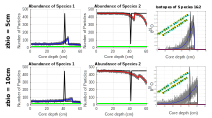
\includegraphics[width=1.0\textwidth]{../figures/1point_event_5+10cm_background.pdf}
	\caption{Example: point event + with background abundance}\label{fig:1pointevent}
\end{center}
\end{figure}


\begin{figure}[hbp]
\begin{center}
	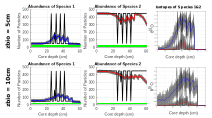
\includegraphics[width=1.0\textwidth]{../figures/../figures/5point_event_5+10cm_background.pdf}
	\caption{Example: 5 point event + with background abundance}\label{fig:5pointevent}
\end{center}
\end{figure}


\begin{figure}[hbp]
\begin{center}
	\includegraphics[width=1.0\textwidth]{../figures/../figures/stepchange2_5+10cm_background.pdf}
	\caption{Example: Step change.}\label{fig:5pointevent}
\end{center}
\end{figure}


\begin{figure}[hbp]
\begin{center}
	\includegraphics[width=1.0\textwidth]{../figures/../figures/stepchange2_5+10cm_background.pdf}
	\caption{Example: Step change.}\label{fig:5pointevent}
\end{center}
\end{figure}


\begin{figure}[hbp]
\begin{center}
	\includegraphics[width=0.8\textwidth]{../figures/../figures/20+40+100kyrcycle_10+20cm_background.pdf}
	\caption{Example: Sine waves.}\label{fig:5pointevent}
\end{center}
\end{figure}


\begin{figure}[hbp]
\begin{center}
	\includegraphics[width=0.8\textwidth]{../figures/../figures/Allcycles_combined_2+5+10+20cm_background.pdf}
	\caption{Example: All cycles combined with z$_\mathrm{bio} \in \{2,5,10,20 \}$cm.}\label{fig:5pointevent}
\end{center}
\end{figure}


\begin{figure}[hbp]
\begin{center}
	\includegraphics[width=1.0\textwidth]{../figures/../figures/Allcycles_combined_pointevent_5+10+20cm_background.pdf}
	\caption{Example: Point event - all cycles combined with z$_\mathrm{bio} \in \{5,10,20 \}$cm.}\label{fig:5pointevent}
\end{center}
\end{figure}
\begin{figure}[hbtp]
\hspace*{-0.8cm}%\caption{Observations from}
\end{figure}

\begin{figure}[hbp]
\begin{center}
	\includegraphics[width=1.0\textwidth]{../figures/../figures/Allcycles_combined_stepevent_bigger_5+10+20cm_background.pdf}
	\caption{Example: Step changes - all cycles combined with z$_\mathrm{bio} \in \{5,10,20 \}$cm.}\label{fig:5pointevent}
\end{center}
\end{figure}



\subsection{Experiments: Only change isotope signal - fixed abundance}
Only the isotopic signal in the forams is changed (same magnitude in both species). Again about 500 total particles are modeled in each layer (now always 350 of species 1 and 150 of species 2). 
After mixing, in order to examine the uncertainties caused by low sample sizes, either 20 or 5 of each foram species are picked in each layer and their isotope values are measured.
Bioturbation depths of 5cm, 10cm and 20cm are used. 

\begin{figure}[hbp]
\begin{center}
	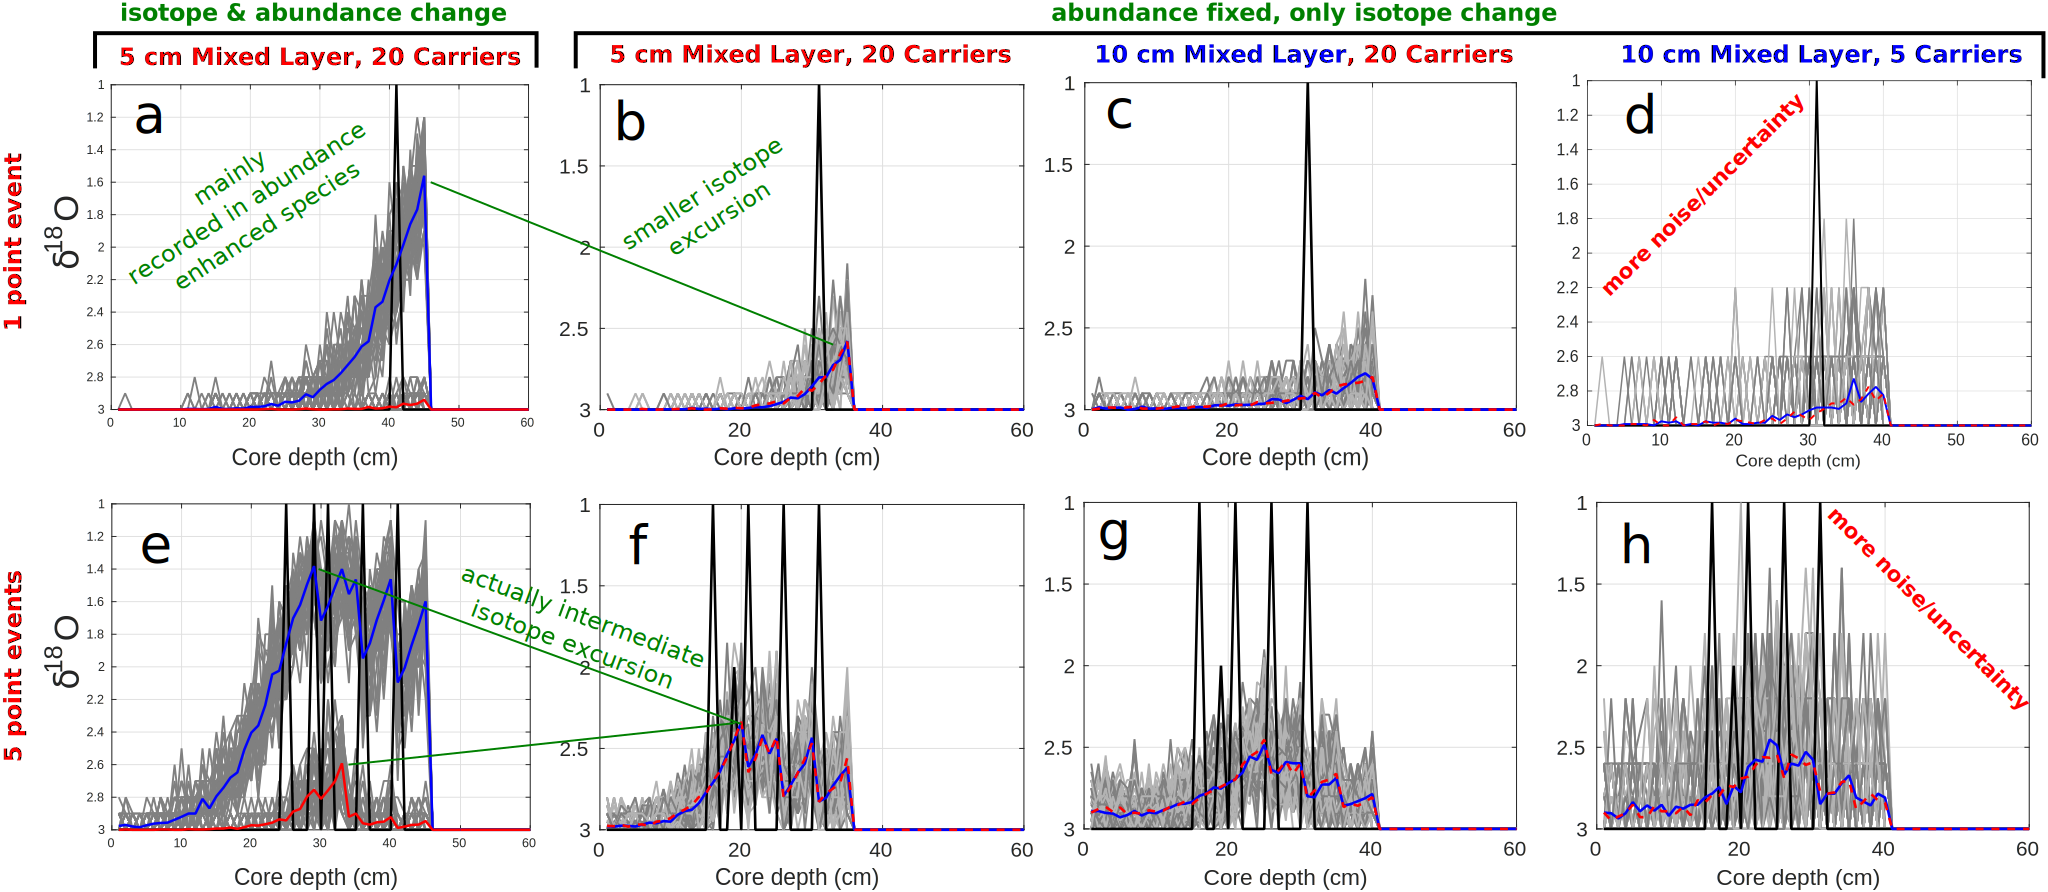
\includegraphics[width=1.0\textwidth]{../figures/../figures/JustABU_pointevent1+5.pdf}
	\caption{Example: Step changes - all cycles combined with z$_\mathrm{bio} \in \{5,10\}$cm and sample size of 20 and 5. }\label{fig:5pointevent}
\end{center}
\end{figure}



\begin{figure}[hbp]
\begin{center}
	\includegraphics[width=1.0\textwidth]{../figures/../figures/JustABU_3ycles_combined.pdf}
	\caption{Example: All cycles combined with z$_\mathrm{bio} \in \{10,20 \}$cm and sample size of 20 and 5. }\label{fig:5pointevent}
\end{center}
\end{figure}

\begin{figure}[hbp]
\begin{center}
	\includegraphics[width=1.0\textwidth]{../figures/../figures/JustABU_3ycles_combined_pointevents.pdf}
	\caption{Example: Point events - all cycles combined with z$_\mathrm{bio} \in \{10,20 \}$cm and sample size of 20 and 5. }\label{fig:5pointevent}
\end{center}
\end{figure}

\begin{figure}[hbp]
\begin{center}
	\includegraphics[width=1.0\textwidth]{../figures/../figures/JustABU_3ycles_combined_gradual.pdf}
	\caption{Example: Step changes - all cycles combined with z$_\mathrm{bio} \in \{10,20 \}$cm and sample size of 20 and 5. }\label{fig:5pointevent}
\end{center}
\end{figure}
\newpage
%% The Bibliography
%% ==> You need a file 'literature.bib' for this.
%% ==> You need to run BibTeX for this (Project | Properties... | Uses BibTeX)
%\addcontentsline{toc}{chapter}{Bibliography} %'Bibliography' into toc
%\nocite{*} %Even non-cited BibTeX-Entries will be shown.
\bibliographystyle{apalike} %Style of Bibliography: plain / apalike / amsalpha / ...
%\bibliography{/home/alex/BRL/bib/literature/VORbib.bib} %You need a file 'literature.bib' for this.
\bibliography{TURBO_050618}


\end{document}
